
% ==============================================================================
%
%                             Introduction
%
% ==============================================================================
\chapter{Introduction}
% Field/Context
Self driving cars are getting more popular and virtual reality video games
increasingly find their way into people's living rooms. One thing they share is
the need for a digital copy of the world. Self driving cars are trained in such
worlds to
accelerate the development of the algorithm and virtual reality games are
becoming more realistic. The Zurich based company Nomoko \cite{nomoko} is developing a
technology that will enable the creation of digital copies of the world. They
built a giga pixel camera and a 3D image processing pipeline to make this happen. This pipeline
consists among other things of high volume image processing. Modern computers
and graphical processing units (GPU) are fast in sequentially processing data
but are designed to serve many different tasks and not a specific one. A
dedicated hardware approach designed for a specific image processing task would
expedite the 3D processing pipeline of creating digital copies of the world.
\\

% Project goal/aims
The goal of this project is to implement such an image processing task on a
Field
Programmable Gate Array (FPGA). FPGAs
consist of thousands of logical elements that can be configured and connected
together to form a complex logical operation. Together with on chip
memory they offer high throughput by processing the data in parallel in contrast to
sequential. The data is transferred to the FPGA over an Ethernet LAN connection
for
fast transfer rates. To accelerate the computing even further, the system needs
to be scalable to multiple FPGA boards to distribute the workload.

% Build upon 
In preparation for this thesis, a semester project focused on two building
blocks for this work: The communication block and the image processing block
\cite{p5report}. The results were two separate parts working but neither
connected nor optimized. This thesis builds upon the results of said work and
focuses on two main goals:

% Primary objectives
\clearpage
\begin{enumerate}
    \item Increase throughput of the dataflow by improving the communication and
    by putting thoughts on scalability
    \item Implement a more complex image processing algorithm to show the real
    benefit of using FPGA for image processing
\end{enumerate}
% \begin{figure}[t!]
%     \centering
%     % \tikzsetnextfilename{system-overview}
\begin{tikzpicture}[
    rounded corners=0mm,
]
    %coordinates
    \coordinate (corig)      at (0,0);
    \coordinate (cmonitor)   at (0,0);
    \coordinate (ccom)       at (5,0);
    \coordinate (cip)        at (10,0);


    %nodes

    \begin{pgfonlayer}{main}
        \node[draw, fill=white, minimum width=3.2cm, minimum height=1.8cm, anchor=west, align=center, rounded corners=1mm] (mon) at (cmonitor) {};

        \node[draw, fill=white, minimum width=2.1cm, minimum height=0.4cm, anchor=west, align=center, rounded corners=2mm, below=0.2cm of mon] (stand) {};
        \node[draw, fill=white, minimum width=0.2cm, minimum height=0.1cm, anchor=south, align=center] (stange) at ($(stand.90) + (0,-0.04)$) {};



        \node[draw, fill=white, minimum width=3cm, minimum height=1cm, anchor=west, text width=2.8cm, align=center, right = 2cm of mon] (com) at (ccom) {Communication};

        \node[draw, fill=white, minimum width=3cm, minimum height=1cm, anchor=west, text width=2.8cm, align=center, right = 1cm of com] (ip) {Image\\Processing};
        

        \node[inner sep=0pt, anchor=west] (whitehead) at ($(cmonitor) + (0.1,0)$)
            {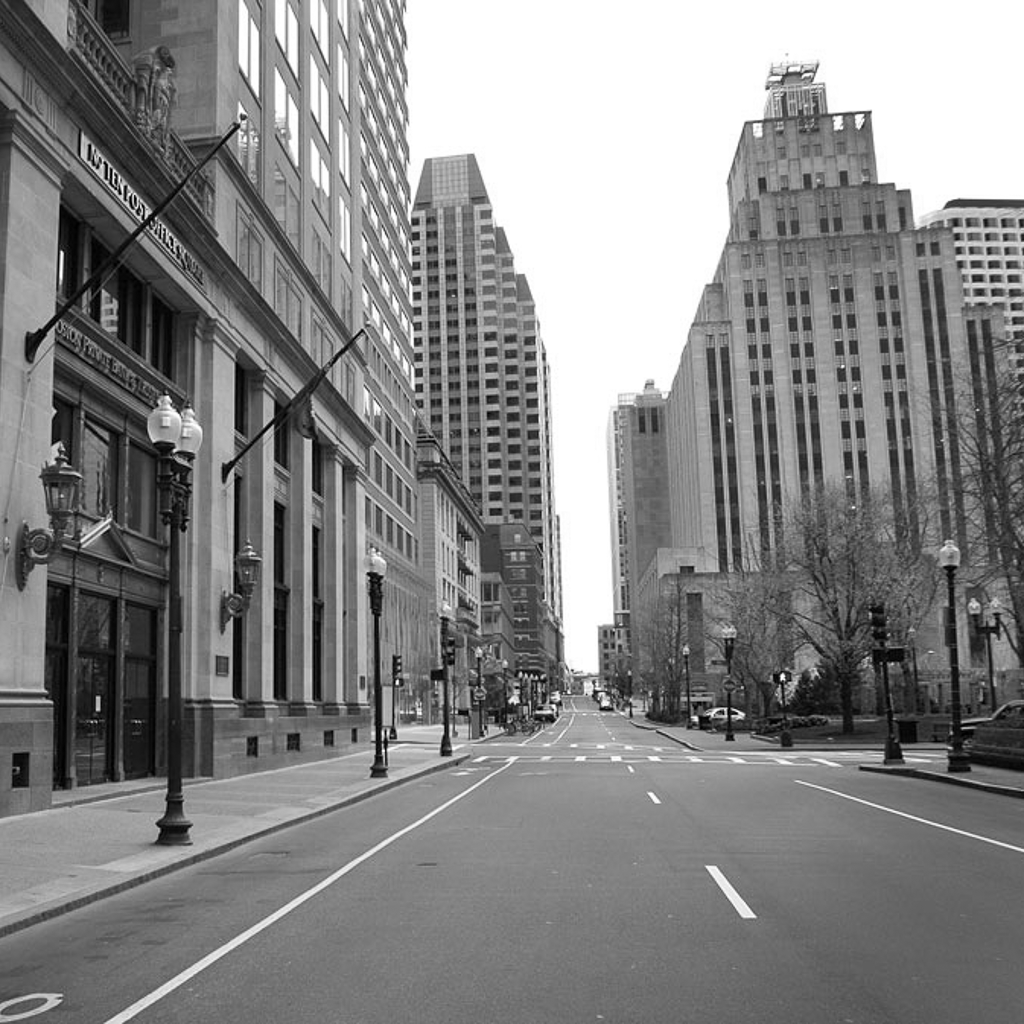
\includegraphics[width=1.4cm]{images/introduction/street1024.png}};
        \node[inner sep=0pt, anchor=west] (whitehead) at ($(cmonitor) + (1.7,0)$)
            {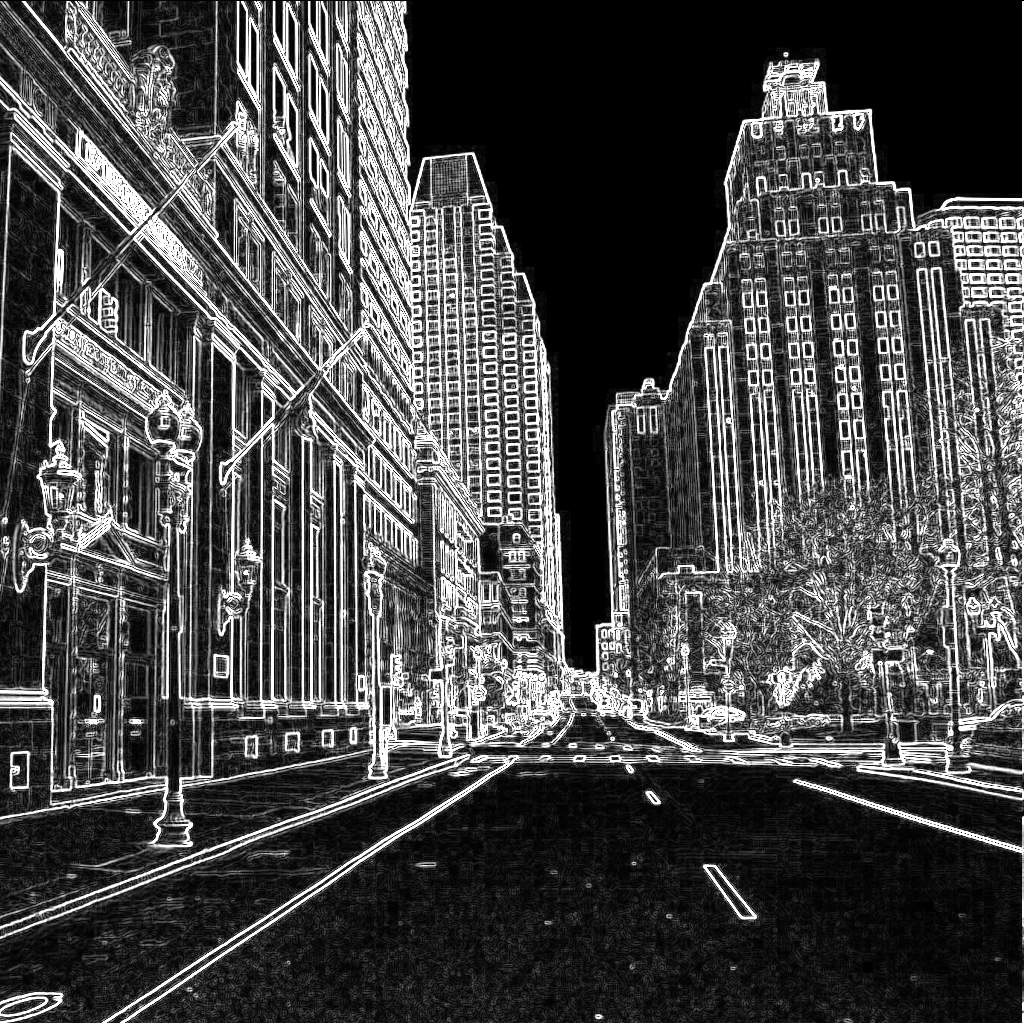
\includegraphics[width=1.4cm]{images/introduction/c_street1024.png}};

        \node[] (eth) at ($(cmonitor) + (4.5, 1.0)$) {LAN};
        
        \draw[line width = 0.5mm] ($(eth) + (0,-1.0)$) ellipse (0.2cm and 0.5cm);
    \end{pgfonlayer}

    % FPGA box
    \begin{pgfonlayer}{main}
        \node[above = 0.2cm of com, xshift=-1.5cm] (fpga) { FPGA };
    \end{pgfonlayer}
    \begin{pgfonlayer}{foreground}
        \node (f_fpga) [draw=black, fill=gray!20, inner sep=20, fit={(com) (ip) }] {};
    \end{pgfonlayer} 

    
    \path[draw,-{Latex[length=2.5mm]}] ($(mon.0) + (0,0.2)$) -- ($(com.180) + (0,0.2)$) node[near end, above] () {1.} ;
    \path[draw,{Latex[length=2.5mm]}-] ($(mon.0) + (0,-0.2)$) -- ($(com.180) + (0,-0.2)$) node[near end, below] () {4.} ;

    \path[draw,-{Latex[length=2.5mm]}] ($(com.0) + (0,0.2)$) -- ($(ip.180) + (0,0.2)$) node[midway, above] () {2.} ;
    \path[draw,{Latex[length=2.5mm]}-] ($(com.0) + (0,-0.2)$) -- ($(ip.180) + (0,-0.2)$) node[midway, below] () {3.} ;

\end{tikzpicture}
%     \caption{Data Flow}
%     \label{fig:datafl}
% \end{figure}

% Sections with NEW are written new in p6
% What is used to realize...
% NEW Dataflow
The existing communication solution is file transfer oriented and stores
received data in memory. This has worked as a proof of concept but is not
optimal
for high throughput image processing. The communication part is extended with an
acknowledge mechanism that allows retransmission of lost packets and a streaming
interface which enables immediate processing of the image data. Furthermore, a
memory management unit is introduced that caches image data to reduce bandwidth
usage.

% NEW Image processing
In the preceding project a Sobel filter was implemented using Vivado HLS. It
uses a simple convolution matrix for edge detection. This operation was well
suited for the first image processing task and to become acquainted with a high
level synthesis tool. For this thesis a new image processing task is realized: the
local contrast enhancement operation called Wallis filter. The algorithm is
described and thoroughly
tested in C/C++ and then synthesized to HDL by the Xilinx Vivado HLS toolchain.
To improve throughput and compare the results of high level synthesis versus a
low level HDL approach, the same filter is implemented in VHDL.

% NEW Scalability
The main intention behind using Ethernet as communication was that the
processing could be distributed onto multiple FPGA. Methods on scalability are
analyzed and compared.

An Artix7 Evaluation Kit by Xilinx serves as a development and testing platform.
It is equipped with gigabit Ethernet LAN and an FPGA with sufficient logic
elements and memory for both the communication and image processing task.
\\

% NEW What is the result of the project
The result is a complete image processing pipeline that begins on a PC where the
input image is sent via Ethernet to the FPGA where it is processed and sent pack
to the PC. The achieved image throughput is 4.1MB/s primarily limited by the image processing core. The Wallis filter core alone
is capable of processing up to 125 megapixels per second on the input. A
benchmark shows the performance differences between a CPU based and FPGA based
solution. 
Concepts on scalability show how the processing power of FPGAs can be
exploited if multiple FPGAs would work on a network. The total throughput then
increases proportional to the number of FPGAs used in the cluster and multiple
gigabytes per seconds of throughput is possible.
\\

% NEW How the document is built up
This report contains six main parts: Theoretical background, mission,
image processing, dataflow, scalability and verification/benchmark.  The
theoretical background explains
the basics of image processing, FPGA, Ethernet communication and on chip
interfaces. The chapter mission will
cover the starting point and presents the concept. Chapters 
image processing and dataflow cover the actual
implementation process of the image processing and dataflow parts.
Before verifying these components in the verification and benchmark chapter the
scalability is studied.

